%!TEX root = Main.tex
\documentclass[Main]{subfiles}

\begin{document}
\section{Theory and Related Works} % (fold)
	\label{sec:theory_and_related_works}
	Humans are very good at discerning emotions in others from looking at pictures or sequences of pictures of faces, among these, the sensation of pain.
	This tells us that there must be visual cues in these, that it is possible to detect and use for classification.

	To find a way of detecting at database of images of people displaying real pain along with reliable labels is needed.
	One such database is the UNBC-McMaster database described in Section \ref{sub:unbc_mcmaster} below.

	\subsection{The UNBC-McMaster Shoulder Pain Expression Archive Database} % (fold)
		\label{sub:unbc_mcmaster}
		The UNBC-McMaster Shoulder Pain Expression Archive Database \cite{Lucey2011} is database of image sequences of subject being observed experiencing pain.
		There are 25 subjects, all suffering from shoulder (rotator cuff) injuries in one shoulder.
		The subjects are asked to move both arms, either manually or by manipulation by a physiotherapist.
		Both arms are moved to provide both positive and negative examples of pain.
		\fxnote{Insert image example of sequences} 

		For each image sequence ie. each movement of an arm, the subjects are asked to report, on a scale of $0-10$, their perceived level of pain.
		An objective observer also evaluates the level of pain the subjects feel.\fxwarning{eh?}
		These are used to control for subjective variances in perception and reporting of pain.
		Both data are available in the database

		From the 25 subjects there are in total 200 sequences, with some subjects having more sequences than others.
		In total there are 48398 frames.
		For each frame facial landmarks are tracked by manually fitting a mask of landmarks to the first frame and then tracking the points throughout the sequence.

		Also for each frame, Action Units (AUs) of the Facial Action Coding System (FACS) \cite{Ekman1978} shown to be related to pain (more on this in Section \ref{ssub:pain_score} below), are evaluated and are available in the database. 
		The FACS AUs each signify a movement or an action of the face eg. the closing of an eye, the raising of an eyebrow or the opening of the mouth.
		The AUs, if present, are all evaluated on a scale of A to E (or somtimes more practically $1-5$) with A meaning \emph{trace} and E meaning \emph{maximum}.

		For a thorough analysis of the database the reader is referred to \cite{Lucey2012}.
		
		\subsubsection{Pain Score} % (fold)
			\label{ssub:pain_score}
			The easiest way of labeling the frames in the UNBC database would be to just label all frames in a sequence with the value i subject reports.
			But there are several problems with this method.
			Firstly there is the problem of individuals experiencing and reporting pain differently, because there are no common reference.
			This can be mediated by using the report of an objective observer, with training in evaluating pain.

			The real problem with the method above is that they assume an equal amount of pain through a whole sequence.
			In reality the level of experienced pain will very throughout the sequence with a peak at some point.
			The level of this peak is then likely what subjects report.
			In order to fully utilize all the image data in the database an indication of pain for each frame is needed.

			\citet{Prkachin1992} have show that there is a high correlation between certain FACS AUs and the level of experienced pain.
			They propose Prkachin and Solomon Pain Intensity (PSPI) score (\ref{eq:PSPI}) as a tool for evaluating pain in subject from their facial expression.
			\begin{equation}
				\label{eq:PSPI} 
				PSPI_{score} = 
					AU4 + \max(AU6,\ AU7) + \max(AU9,\ AU10) + AU43
			\end{equation}
			The Action Units account for brow lowering (AU4), orbital tightening (AU6 and AU7),levator contraction (AU9 and AU10) and eye closure (AU43).
			The values are numerical (0 = absent, 5 = maximum).
			The value for eye closure (AU43) is binary (0 = open, 1 = closed).
			This gives the score a scale of $0-16$.

			Because FACS codes are available for each frame, the PSPI score is a good choice for labeling data at the frame level.
			This is further supported by that fact that we know that the emotions felt in the experiment is pain.
			Therefore we can with high probability attest the AUs to the pain and not other factors/emotions.

			% subsubsection pain_score (end)

		\subsubsection{Problems With Using the UNBC Database} % (fold)
			\label{ssub:problems_with_using_the_unbc_database}
			The UNBC database is a good and important tool for the development of pain recognition systems.
			It does however leave one wanting at some points.

			Firstly, of the 48398 frames in the database 40029 are frames with no pain at all.
			And of the ones showing pain most are very low levels (see Figure \ref{fig:HistogramOfPain}).
			This results is a high a priori probability of no pain in the data.

			\begin{figure}[H]
				\centering 
				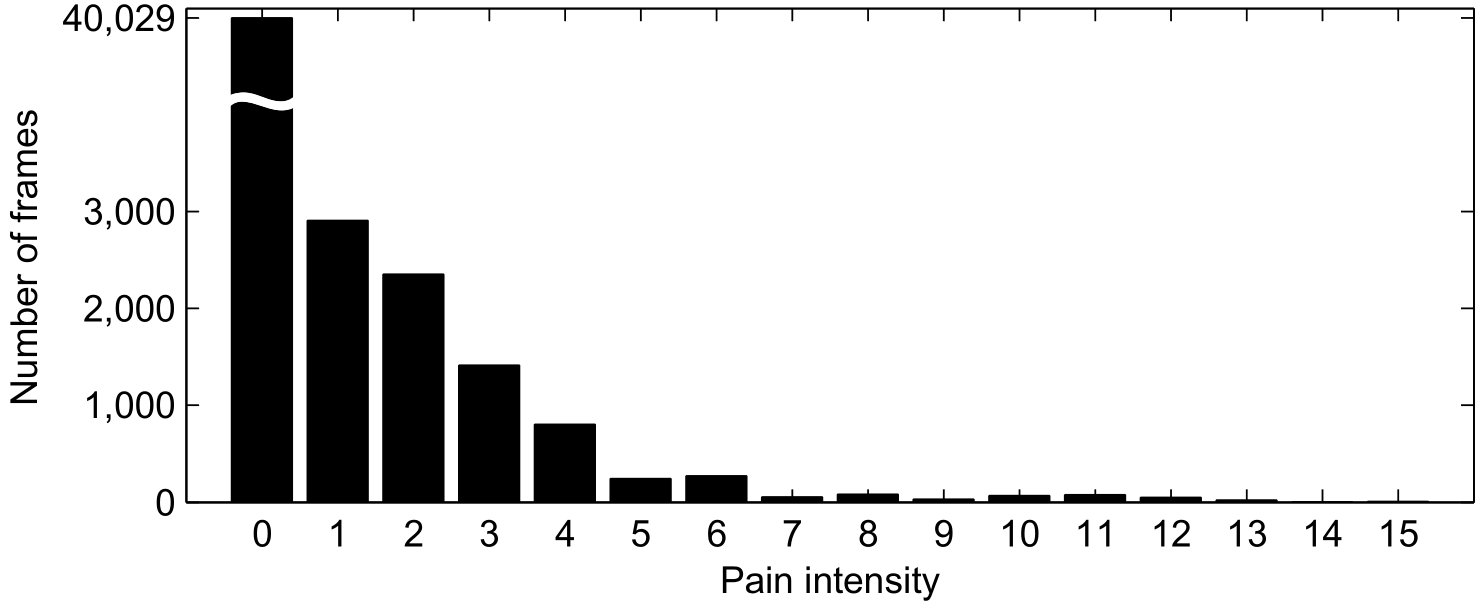
\includegraphics[width=\textwidth]{HistogramOfPain}
				\caption{
					Histogram of PSPI scores in UBNC database. 
					Figure taken from \cite{Kaltwang2012}
					}
				\label{fig:HistogramOfPain}
			\end{figure}

			Secondly, the database only show subject in pain.
			This means that without negative examples of other than neutral faces, there is a risk of over-fitting certain features that may be more generally show for a wider range of emotions, leading to false positives.
			A solutions to this could be as in \cite{florealearning}, where the authors use the UNBC database to learn specific pain related features, but also the more general \emph{Cohn-Kanade AU-Coded Expression Database} \cite{Kanade2000} to ensure better generalization of their model.
			Such an approach is however beyond the scope of this report.

			Finally, there is a lot of frames in the database in which the subjects turn or bow their heads enough to interfere with the processing and classification.
			This is also documented in \cite{Lucey2012}.
			The problem is that this was not monitored/recorded in the creation of the database, so it hard to automatically adjust for or ignore.
			Estimating head pose and correcting for this like in \fxerror{insert citation} is beyond the scope of this report.



			% subsubsection problems_with_using_the_unbc_database (end)

		% subsection unbc_mcmaster_schoulder_pain_database (end)

	\subsection{Related Works} % (fold)
		\label{sub:related_works}	

		\fxnote{More articles?}

		
		\fxerror{something that ties this to the work on the database mentioned above}
		In \cite{Lucey2011} the creators of the UNBC database use the registered landmarks in the images to make procrustes aligned representations of the faces along with facial appearance, shape normalized using Active Shape Models (ASM) and Active Appearance Models (AAM), as feature vectors.
		These feature vectors are then used to train a Support Vector Machine (SVM).
		With this they achieved detection rates of $57.1\%$ to $87.5\%$ for individual FACS AUs and up to $83.9\%$ for binary pain detection.

		In this report I attempt to reproduce these results using the same data and with a similar approach but with my own implementation.

		\fxwarning{painful face article to support the above mentioned claim}

		\citet{Kaltwang2012} similarly use the UNBC database.
		They compare the performance of using shape based features (PTS), taken from the registered landmarks, with appearance features.
		The appearance feature were both 2D Discrete Cosine Transform (DCT) and Local Binary Patterns (LBP).
		The authors employ Relevance Vector Regression (RVR) to estimate pain for type of feature (shape, DCT and LBP).
		A fusion of the individual features pain estimates is then made, again using RVR.
		The authors conclude that appearance based features outperform shape based.
		They do however believe that improved registration of shape, that compensates for out of plane motion (eg. \cite{Rudovic2011}), would improve performance.
		Regarding the appearance based feature, the authors state that in most cases the LBP features worked better than DCT features, taken individually.

		A major shortfall of the methods described above is that they all \fxnote{Check if this is true when other articles are added} rely on the facial landmarks that are registered with human intervention.
		Without self implementing a strong and reliable way of automatically registering these, systems like the ones described above are not applicable for use in real-life, real-time applications.
		Therefore I try a completely different approach in this report.

		An inspiration for this approach is \cite{Shen2012a}.
		In this, the authors predict human eye fixation using deep Convolutional Neural Networks to extract high level features. 
		This approach does not use human selected features, but instead uses human eye tracking data to learn the high level features that humans fixate on.
		A similar approach could possibly be tuned to register the same cues that humans use to recognize pain in faces.

		% subsection related_works (end)

	\subsection{Proposed approach} % (fold)
		\label{sub:proposed_approach}
		The novel approach in this project is to use only the image data from the UNBC database as input data and only use the metadata for ground truth labeling of the training, test and validation data.

		The method can be summarized as follows:
		\begin{enumerate}
			\item 
			A Viola-Jones detector \fxnote{Reference?} will be used to locate the face in the images.
			
			\item 
			A patch around the face will be extracted.

			\item
			The extracted patch will be resized to a fixed size eg. $100 \times 100$ or $48 \times 48$ pixels.

			\item
			The resized patches will be used to train a Convolutional Neural Network (CNN)

		\end{enumerate}

		Several ideas for the scope of each classification network exist.
		One idea is to train a large network with all the data on all types of subject, to have a very generalized model.

		Another is to train a couple of networks one a few stereotypes of subjects ie. males, females, children and perhaps also different age segments separately. This would be less general, but maybe better tuned to the idiosyncrasies of each group.

		A final idea is to train a model on a per subject basis.
		This would likely not generalize very well to all other subjects.
		Instead it may be better equipped to handle the sometimes very individual response of subjects to certain levels of pain.
		\fxnote{Make sure to include something about handicapped/paralyzed subjects} 
		This idea may be especially relevant in cases with subjects who are mentally handicapped or paralyzed, as their response patterns related to pain are know to deviate from the norm.\fxnote{Reference}
		For this to work though, it would require that it is possible to train the network with few enough data, that it would be feasible to acquire for each subject.
		A way of achieving this would be to refine a more general pre-trained network.


		% subsection proposed_approach (end)
	
	% section theory_and_related_works (end)

\end{document}
